%\listfiles
\documentclass[tg]{mdtufsm}
% um tipo específico de monografia pode ser informado como parâmetro opcional:
%\documentclass[tese]{mdtufsm}
% a opção `openright' pode ser usada para forçar inícios de capítulos
% em páginas ímpares
% \documentclass[openright]{mdtufsm}
% para gerar uma versão frente-e-verso, use a opção 'twoside':
% \documentclass[twoside]{mdtufsm}

\usepackage[T1]{fontenc}        % pacote para conj. de caracteres correto
\usepackage{fix-cm} %para funcionar corretamente o tamanho das fontes da capa
\usepackage{times, color, xcolor}       % pacote para usar fonte Adobe Times e cores
\usepackage[utf8]{inputenc}   % pacote para acentuação
\usepackage{graphicx}  % pacote para importar figuras
\usepackage{amsmath,latexsym,amssymb} %Pacotes matemáticos
\usepackage[%hidelinks%, 
            bookmarksopen=true,linktoc=none,colorlinks=true,
            linkcolor=black,citecolor=black,filecolor=magenta,urlcolor=blue,
            pdftitle={Desenvolvimento de um escalonador sensível ao contexto para o Apache Hadoop},
            pdfauthor={Guilherme Weigert Cassales},
            pdfsubject={Trabalho de Graduação},
            pdfkeywords={Apache Hadoop, escalonador, sensível ao contexto, Informática, UFSM}
            ]{hyperref} %hidelinks disponível no pacote hyperref a partir da versão 2011-02-05  6.82a
%Nesse caso, hidelinks retira os retângulos em volta dos links das referências

%Margens conforme MDT 7ª edição, arrumar diretamente no mdtufsm.cls para funcionar a opção twoside *PENDENTE*
\usepackage[inner=30mm,outer=20mm,top=30mm,bottom=20mm]{geometry} 
\usepackage{epstopdf}
\usepackage{graphicx}


%==============================================================================
% Se o pacote hyperref foi carregado a linha abaixo corrige um bug na hora
% de montar o sumário da lista de figuras e tabelas
% Se o pacote não foi carregado, comentar a linha %
%==============================================================================

%%=============================================================================
%% Trampa para corrigir o bug do hyperref que redefine o caption das figuras e das
%% tabelas, n�o colocando o nome ``Figura'' antes do n�mero do mesmo na lista
%%=============================================================================

\makeatletter

\long\def\@caption#1[#2]#3{%
  \expandafter\ifx\csname if@capstart\expandafter\endcsname
                  \csname iftrue\endcsname
    \global\let\@currentHref\hc@currentHref
  \else
    \hyper@makecurrent{\@captype}%
  \fi
  \@ifundefined{NR@gettitle}{%
    \def\@currentlabelname{#2}%
  }{%
    \NR@gettitle{#2}%
  }%
  \par\addcontentsline{\csname ext@#1\endcsname}{#1}{%
    \protect\numberline{\csname fnum@#1\endcsname ~-- }{\ignorespaces #2}%
  }%
  \begingroup
    \@parboxrestore
    \if@minipage
      \@setminipage
    \fi
    \normalsize
    \expandafter\ifx\csname if@capstart\expandafter\endcsname
                    \csname iftrue\endcsname
      \global\@capstartfalse
      \@makecaption{\csname fnum@#1\endcsname}{\ignorespaces#3}%
    \else
      \@makecaption{\csname fnum@#1\endcsname}{%
        \ignorespaces
        \ifHy@nesting
          \expandafter\hyper@@anchor\expandafter{\@currentHref}{#3}%
        \else
          \Hy@raisedlink{%
            \expandafter\hyper@@anchor\expandafter{%
              \@currentHref
            }{\relax}%
          }%
          #3%
        \fi
      }%
    \fi
    \par
  \endgroup
}

\makeatother

%==============================================================================
% Identificação do trabalho
%==============================================================================
\title{Desenvolvimento de um escalonador sensível ao contexto para o Apache Hadoop}

\author{Cassales}{Guilherme Weigert}

\course{Curso de Ciência da Computação}
\altcourse{Curso de Ciência da Computação}

\institute{Centro de Tecnologia}
\degree{Bacharel em Ciência da Computação}

% Número do TG (verificar na secretaria do curso)
% Para mestrado deixar sem opção dentro do {}
\trabalhoNumero{}

%Orientador
\advisor[Profª.]{Drª.}{Charão}{Andrea Schwertner}
%Se for uma ``orientadora'' descomentar a linha baixo
\orientadoratrue

%Avaliadores (Banca)
\committee[Prof. Dr.]{Stein}{Benhur de Oliveira}{UFSM}
\committee[Profª. Drª.]{Barcelos}{Patrícia Pitthan de Araújo}{UFSM}


% a data deve ser a da defesa; se nao especificada, são gerados
% mes e ano correntes
\date{13}{Novembro}{2013}

%Palavras chave
\keyword{Apache Hadoop} 
\keyword{Escalonador}
\keyword{Sensibilidade ao Contexto}

%%=============================================================================
%% Início do documento
%%=============================================================================
\begin{document}

%%=============================================================================
%% Capa e folha de rosto
%%=============================================================================
\maketitle

%%=============================================================================
%% Catalogação (obrigatório para mestrado) e Folha de aprovação
%%=============================================================================
%Somente obrigatório para dissertação, para TG, remover as linhas	77	%
%Como a CIP vai ser impressa atrás da página de rosto, as margens inner e outer	
%devem ser invertidas.
%\newgeometry{inner=20mm,outer=30mm,top=30mm,bottom=20mm}	
%\makeCIP{nomedoautor@gmail.com} %email do autor		
%\restoregeometry

%Se for usar a catalogação gerada pelo gerador do site da biblioteca comentar as linhas
%acima e utilizar o comando abaixo
%\includeCIP{CIP.pdf}

%folha de aprovação
\makeapprove


%%=============================================================================
%% Resumo
%%=============================================================================
\begin{abstract}

Hoje em dia, o volume de dados gerados é muito maior do que a capacidade de processamento dos computadores. Como solução para esse problema, algumas tarefas podem ser paralelizadas ou distribuidas. O \emph{framework Apache Hadoop} \cite{Hadoop}, é uma delas e poupa o programador as terefas de gerenciamento, como tolerância à falhas, particionamento dos dados entre outros.
Um problema no escalonador do \emph{Apache Hadoop} é que seu foco é em ambientes homogêneos, o que muitas vezes não é possível de se manter. O foco deste trabalho é implementar um novo escalonador que seja sensível ao contexto e que leve em conta as capacidades físicas de cada máquina na hora de distribuir as tarefas submetidas.

Nowadays the volume of data generated by the services provided for end users, is way larger than the processing capacity of one computer alone. As a solution to this problem, some tasks can be parallelized. The Apache Hadoop framework \cite{Hadoop}, is one of these parallelized solutions and it spares the programmer of management tasks such as fault tolerance, data partitioning, among others.
One problem on this framework is the scheduler, which is designed for homogeneous environments. It is worth to remember that maintaining a homogeneous environment is somewhat difficult today, given the fast development of new, cheaper and more powerful hardware. This work focuses on altering the Capacity Scheduler, in order to make it more context-aware towards resources on the cluster since, the original scheduler assumes that every node on cluster has the same amount of memory and therefore may set the resources too high or too low. 
This work managed to insert code on NodeManager methods so that it will collect data on every node and send it to CapacityScheduler, which will adjust the allocation values according to the total cluster resources.






\end{abstract}


%% Lista de Ilustrações (opc)
%% Lista de Símbolos (opc)
%% Lista de Anexos e Apêndices (opc)

%%=============================================================================
%% Lista de figuras (comentar se não houver)
%%=============================================================================
%%\listoffigures

%%=============================================================================
%% Lista de tabelas (comentar se não houver)
%%=============================================================================
%%\listoftables

%%=============================================================================
%% Lista de Apêndices (comentar se não houver)
%%=============================================================================
%\listofappendix

%%=============================================================================
%% Lista de Anexos (comentar se não houver)
%%=============================================================================
%\listofannex

%%=============================================================================
%% Lista de abreviaturas e siglas
%%=============================================================================
 %o parametro deve ser a abreviatura mais longa
%\begin{listofabbrv}{UbiComp}
%   \item [BNF] \textit{Backus-Naur Form}
%   \item [UbiComp] Computação Ubíqua
%\end{listofabbrv}


%%=============================================================================
%% Lista de simbolos (opcional)
%%=============================================================================
%Simbolos devem aparecer conforme a ordem em que aparecem no texto
% o parametro deve ser o símbolo mais longo
%\begin{listofsymbols}{teste}
%  \item [$\varnothing$] vazio
%  \item [$\Gamma$]  Gama
%  \item [$\forall$] Para todo
%\end{listofsymbols}

%%=============================================================================
%% Sumário
%%=============================================================================
\tableofcontents


%%=============================================================================
%% Início da dissertação
%%=============================================================================
\setlength{\baselineskip}{1.5\baselineskip}

%Adiciona cada capitulo
\chapter{Introduction}
\label{chap:Introduction}
One of the major IT companies nowadays, known as Google \cite{Google}, had the initial idea of a way to process a huge data volume generated by its servers. This approach would later be known as MapReduce, built by two separate steps, Map and Reduce, each step based on a functional language function. At the same time, a Yahoo! \cite{Yahoo} led project was starting the implementation of MapReduce for its own system, which would then become a whole new project, named Apache Hadoop \cite{Hadoop}.

Today the Apache Hadoop framework has a very active community of both developers and users, however there are some characteristics that weren't changed from the day the framework was first designed. Among these characteristics there is one very detrimental and prone to bad performance issues, which is the focus on homogeneous environments. It is known that maintaining a totally homogeneous environment is harder and harder as the time passes, requiring either a huge initial investment or a huge effort in order to replace faulty hardware without changing the component capability.

The MapReduce's task performance inside Hadoop is tightly tied to the scheduler \cite{CASH}. Since it is an open source project, it is possible to change the scheduler aiming to make it capable of better adapting to heterogeneity while at the same time presenting a performance improvement.

A key characteristic in Hadoop's transition to heterogeneous environments is the context-aware capability. The definition of context can vary from one application to another, but as a rule of thumb it is some information that the application can use as base for decision making. When an application is context-aware, it will detect and adapt to the changes in the environment \cite{Manuele}.

In the present work, the context to which the application will have to adapt is related to the physical configuration of the machines that compose the Hadoop cluster, allowing the scheduler to work with real data collected from the machines and not suppositions as the default Hadoop configuration implies. In a more complex degree, the present work is just a part of a bigger project called PER-MARE \cite{PER-MARE}, which has the objective of adapting to more environment variations, as the insertion and removal of nodes in real time.


%-------------------------------------------------------------------
\section{Objective}

The main objective of this work is to improve Hadoop through a context-aware scheduling, which will provide better performance and adaptation on heterogeneous environments.

%-------------------------------------------------------------------
\section{Motivation}

Today, some processing tasks that used to be made through huge mainframes and servers are gradually transitioning to big clusters, which are composed of computers with more accessible prices and easily bought in the market. 

Even though the Apache Hadoop framework has clusters as its target, it was designed and implemented under a specific assumption. The framework's better performance is achieved when it is running on a homogeneous cluster, in other words, when all nodes have the same resources. The problem is that given today's hardware development, it might take the system to a point where it is not possible or at least not profitable to maintain cluster homogeneity. 

Since the default configuration of the scheduler tells that every node on the cluster has the same amount of resources, if a more powerful node is inserted all that extra capacity will be wasted. This happens because the cluster will not collect the real configuration, but the parameter set in a XML file as the node capacity. The opposite is also troublesome, if a less powerful node is inserted, the cluster will use it as if it had more potential, possibly overloading that node with more tasks that it can handle and causing errors or performance issues.

The present work is relevant, as it's objective is based on adaptation and improvement of an already existent technology. With the improved scheduler, not only will the Apache Hadoop clusters have a possibility to improve cluster's resource utilization, as the framework itself will be better prepared and capable of adapting to new heterogeneous environments in an easier and smoother way.
\chapter{Fundamentos e Revisão de Literatura}
\label{chap:fundamentacao}
É necessário definir alguns termos, técnicas e/ou ferramentas para o entendimento deste trabalho. Por exemplo, a conceituação formal de sensibilidade ao contexto é muito importante, uma vez que constitue-se da técnica de obtenção dos dados. Como complemento à sensibilidade ao contexto define-se o que é o ZooKeeper, a ferramenta utilizada para transmissão dos dados coletados. Além disso, é relevante que exista a compreensão de como o Apache Hadoop, seu escalonamento e o paradigma de programação utilizado funcionam, bem como quais trabalhos já foram feitos neste âmbito.

%-------------------------------------------------------------------

\section{Sensibilidade ao Contexto}
\label{sec:ctx}
Quando um usuário acessa um site por meio de um dispositivo móvel este site carrega automaticamente sua versão \emph{mobile}, a qual possui alterações que aumentam a compatibilidade com o tipo de dispositivo sendo utilizado. Uma situação semelhante ocorre quando navegadores utilizam dados de localidade para melhorar os resultados de um motor de buscas, mostrando primeiro os resultados mais relacionados com a região ou idioma do usuário. Nota-se que nas duas situações a aplicação utiliza dados específicos, o tipo do dispositivo e a localização do usuário, coletados no momento da execução e utiliza-os para adaptar o seu funcionamento de maneira a oferecer maior conforto ou usabilidade ao usuário. Estes dados representam o contexto dos usuários, o qual é definido por \cite{Dey} como qualquer informação que pode ser utilizada para caracterizar a situação de uma entidade (pessoa, lugar ou objeto) considerada relevante para a interação entre usuário e aplicação.

Sendo assim, se uma aplicação é capaz de coletar informações sobre a situação do sistema no qual está sendo executada, ela é capaz de coletar informações de contexto. Porém a simples coleta não aumenta, de fato, o desempenho desta aplicação, é necessário que ela seja capaz de responder às mudanças do ambiente detectadas. Esta capacidade de detecção e reação é caracterizada como sensibilidade ao contexto por \cite{Maamar} e vai ao encontro da definição de \cite{Baldauf} em que o sistema deve detectar mudanças e adaptar suas operações sem intervenção explícita do usuário, aumentando assim a usabilidade e eficácia da aplicação.


%-------------------------------------------------------------------

\section{Hadoop}
O \textit{framework} Apache Hadoop origina-se de outro projeto da Apache, o Apache Nutch \cite{Nutch}. O Apache Nutch iniciou em 2002 como um motor de buscas de código livre, porém o projeto encontrou problemas devido a sua arquitetura. Quando a Google publicou um artigo em 2003 descrevendo a arquitetura utilizada no seu sistema de arquivos distribuídos, chamado GFS (\textit{Google File System}), os desenvolvedores do Nutch notaram que uma arquitetura semelhante resolveria seus problemas de escalabilidade. A implementação da ideia foi iniciada em 2004 e o resultado foi nomeado \textit{Nutch Distributed Filesystem} (NDFS). Contudo, a medida em que o projeto se desenvolvia o propósito original do Nutch era deixado em segundo plano, o que culminou na criação de um novo projeto em 2006. Este novo projeto foi nomeado Apache Hadoop e possui o propósito de facilitar o processamento distribuído através do paradigma MapReduce.

\subsection{Arquitetura geral do \emph{Apache Hadoop}}
O \textit{framework} Apache Hadoop é organizado em uma arquitetura de mestre-escravo e possui dois serviços principais, o serviço de armazenamento (HDFS - Hadoop Distributed File System) e o de processamento (YARN - Yet Another Resource Negotiator), os quais podem ser vistos na Figura \ref{fig:ArquiteturaHadoop}.

\begin{figure}[!ht]
\centering
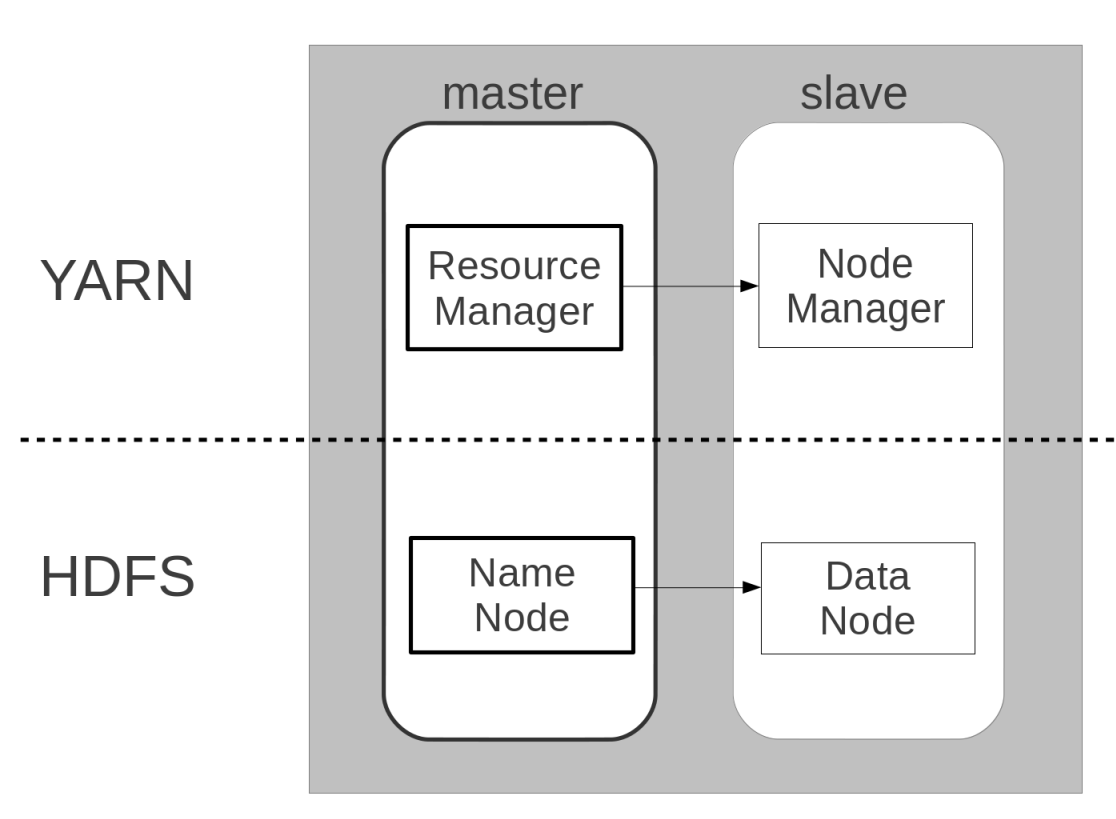
\includegraphics[width=0.7\textwidth]{figuras/Figura08-HadoooArchGeral.png}
\caption{Arquitetura geral do Apache Hadoop}
\label{fig:ArquiteturaHadoop}
\end{figure}

Nesta figura, é possível notar a existência de 4 componentes do \textit{framework}. Os componentes acima da linha pontilhada pertencem ao YARN, sendo o Resource Manager e o Node Manager os serviços mestre e escravo respectivamente. O HDFS é composto pelos componentes abaixo da linha pontilhada, sendo o Name Node e o Data Node os serviços mestre e escravo respectivamente.

\subsubsection{HDFS}
Grande parte do ganho de desempenho oferecido pelo Hadoop decorre do comportamento de levar o processamento até os dados, ou seja, todo processamento é feito com dados locais. Esta abordagem só é possível de ser realizada graças ao HDFS. Dentro do Name Node são mantidas informações de quais partes de quais arquivos estão em cada Data Node, ou seja, todos os arquivos estão divididos num grande HD distribuído e o mestre sabe exatamente quais blocos cada escravo possui. Dessa forma cada nó executa tantos Maps ou Reduces quanto a quantidade de arquivos locais permitir, diminuindo a necessidade de utilizar a rede para transferência de arquivos e deixando-a disponível para ser utilizada para a transferência dos resultados que são os dados já reduzidos. Um problema dessa abordagem é que o Hadoop possui uma latência muito alta, sendo desaconselhável o uso do Hadoop em aplicações críticas ou de tempo real \cite{BookHadoop}. A Figura \ref{fig:ArqHDFS} apresenta um esquema básico da arquitetura do HDFS.

\begin{figure}[!hbtn]
   \centering
   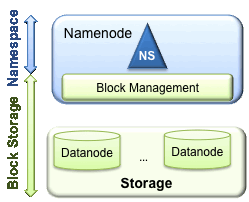
\includegraphics[width=8cm]{figuras/Figura07-HDFS.png}
   \caption{Arquitetura geral do HDFS \cite{HDFS}}
   \label{fig:ArqHDFS}
\end{figure}

\subsubsection{YARN}
Sendo o componente do Apache Hadoop responsável pela execução do \emph{MapReduce}, o YARN realiza tarefas de gerenciamento e execução do processamento. Um dos objetivos do YARN é tornar a tarefa de processamento totalmente independente das tarefas de armazenamento, possibilitando que o \textit{cluster} seja utilizado em conjunto com outras ferramentas que não utilizem o paradigma MapReduce \cite{Vavilapalli}. A Figura \ref{fig:ArqYARN} apresenta um esquema básico da arquitetura do YARN.

\begin{figure}[!hbtn]
   \centering
   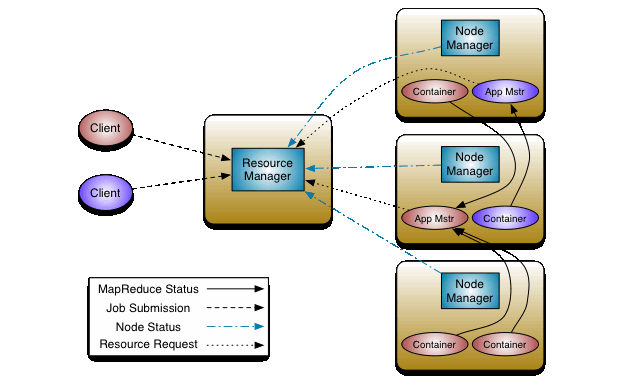
\includegraphics[width=12cm]{figuras/Figura06-YarnArch.png}
   \caption{Arquitetura geral do YARN \cite{YARN}}
   \label{fig:ArqYARN}
\end{figure}

Na imagem é possível observar dois novos componentes do YARN. O primeiro é um componente do Node Manager, possuindo o papel de um escalonador interno de cada aplicação (Application Master - referenciado na imagem como App Mstr), sendo também conhecido por escalonador de tarefas. Considera-se que tarefas sejam uma fração do processamento das aplicações, ou seja, cada tarefa de Map ou Reduce corresponde a uma das divisões que serão processadas em paralelo. É importante não confundir este componente com o escalonador de aplicações, o qual é um componente do Resource Manager e pode ser melhor compreendido com a leitura da Seção \ref{sec:HadSched}. O outro componente presente na figura é o Container, o qual representa uma alocação de recursos em um nó qualquer do \textit{cluster}. A importância do container vem do fato de que todas as tarefas são executadas em uma instância de container.

É importante notar que existem 2 instâncias de Application Master na figura e que elas estão, assim como os clientes e os containers, coloridas de rosa ou roxo para indicar que pertencem à mesma aplicação, ou seja, o cliente rosa lançou uma aplicação que possui o Application Master e mais 3 containers de processamento. Nota-se também que o Resource Manager recebe informações tanto dos clientes quanto dos Node Managers e Application Masters, centralizando todas elas para um controle dos recursos disponíveis.

\subsection{Configuração do ambiente de execução do Hadoops}
Uma característica importante do Hadoop tem relação com sua configuração. Sabe-se que todo sistema necessita de uma configuração por parte de seu administrador, e o Hadoop não é diferente com relação a isso. O Hadoop utiliza uma série de arquivos em cada um dos nós do \textit{cluster} para definir sua configuração. Estes arquivos de configuração são, na verdade, arquivos XML compostos por parâmetros de configuração e valores que influenciam o comportamento do \textit{framework} no \textit{cluster}. Para conhecimento, esses arquivos são: \textit{core-site.xml, yarn-site.xml, mapred-site.xml} e \textit{hdfs-site.xml}. Cada um destes arquivos possui propriedades de um serviço do Hadoop, como exemplo o arquivo \textit{hdfs-site.xml} é responsável pela configuração do HDFS na máquina em questão. 

É importante salientar que para a execução distribuída, ao menos algumas propriedades mais simples dos arquivos de cada nó, seja este mestre ou escravo, devem ser configuradas. No caso do administrador desejar fazer uma configuração mais específica de cada nó escravo ele deverá editar as propriedades nos arquivos de cada um dos nós. Caso o administrador não queira configurar os nós escravos, eles irão executar com base nos valores \textit{default}, contudo esta decisão irá, provavelmente, afetar o desempenho do \textit{cluster} devido à má configuração.

\section{MapReduce}
O paradigma de programação MapReduce é, geralmente, associado com implementações que processam e geram grandes conjuntos de dados. Neste paradigma, todo processamento é dividido em duas etapas, a etapa de Map e a de Reduce, originárias das linguagens funcionais. Como consequência da divisão em duas etapas, o resultado da primeira é a entrada da segunda e esta transferência de dados é baseada em de pares de chave e valor, o que torna possível expressar uma vasta gama de tarefas reais por meio deste paradigma \cite{Dean}.

O \textit{work-flow} padrão de uma aplicação MapReduce inicia com a entrada de dados, que será dividida em \textit{n} partes e cada parte será processada individualmente por uma tarefa Map. O resultado das tarefas Map já será na forma de pares chave e valor, que serão passados como entrada para as tarefas de Reduce. Por sua vez, as tarefas de Reduce irão receber todos os pares com determinada chave e aplicar um algoritmo sobre os pares, fornecendo uma saída inteligível \cite{BookHadoop}.

%TODO citação
A naturalidade do paralelismo deste paradigma, torna a programação da aplicação mais simples. Ao utilizar o paradigma do MapReduce o programador deve apenas pensar em uma solução que siga o \textit{work-flow} do paradigma, e o parelelismo será inerente.

\section{ZooKeeper}
O ZooKeeper é um projeto da Apache e fornece ferramentas eficientes, confiáveis e tolerantes à falha para a coordenação de sistemas distribuídos \cite{Hunt2010}. Inicialmente, o ZooKeeper foi implementado como um componente do Hadoop e virou um projeto próprio conforme cresciam suas funcionalidades e sua utilização em outras aplicações. 

A arquitetura utilizada no ZooKeeper é a de cliente-servidor, sendo o servidor o próprio ZooKeeper (chamado de \textit{ensamble}), enquanto a aplicação que o está utilizando assume o papel de cliente. A maneira como os clientes interagem depende da aplicação.

Os dados do ZooKeeper ficam armazenados em \textit{zNodes}, abstrações que podem ser tanto um \textit{container} de dados quanto de outros \textit{zNodes}, e formam um sistema de arquivos hierárquico que pode ser comparado à estrutura de uma árvore. Para garantir a consistência deste sistema de arquivos o ZooKeeper utiliza operações de escrita linearizáveis, as quais são obrigatoriamente processadas pelo servidor líder que é, então, encarregado de propagar as mudanças para os demais participantes do \textit{ensamble} \cite{Pham}.

Um dos principais recursos do ZooKeeper são os \textit{Watchers}, interfaces providas pelo \textit{framework} que permitem aos clientes monitorarem certos \textit{zNodes}. Quando um \textit{Watcher} é registrado como monitor de um \textit{zNode}, ele pode ser configurado para monitorar a alteração dos dados do \textit{zNode}, a criação/remoção de \textit{zNodes} filhos, ou ainda para qualquer tipo alteração no \textit{zNode} e seus filhos. Quando um \textit{zNode} sofre uma alteração que o \textit{Watcher} está monitorando uma \textit{callback} é disparada para que o cliente faça o processamento desejado \cite{HadoopBook}.

No âmbito deste trabalho, os serviços do ZooKeeper são utilizados para monitorar as informações de contexto coletadas nos nós escravos e transmiti-las para o escalonador. Sendo que a comunicação é feita através de processos que atualizam e monitoram o conteúdo de \textit{zNodes}.


%-------------------------------------------------------------------

\section{Escalonadores para o Hadoop}
\label{sec:HadSched}
Apesar de existirem dois níveis de escalonamento no Hadoop, escalonamento de aplicações e de tarefas, este trabalho influencia apenas o escalonamento de aplicações. O escalonador de aplicações gerencia qual será a primeira aplicação a receber um \textit{container} para seu escalonador de tarefas e quais serão os escalonadores de tarefa que receberão recursos para execução \cite{BookHadoop}. O Hadoop já inclui alguns escalonadores que oferecem maneiras diferentes para a realização do escalonamento de aplicações. Para alterar o escalonador utilizado é necessário alterar uma propriedade no arquivo \textit{yarn-site.XML} e reiniciar o Resource Manager.

Dentre os escalonadores incluídos no Hadoop, o mais simples é o Hadoop Internal Scheduler que utiliza o algoritmo FIFO e tem boa performance em \textit{clusters} onde não existe competição por recursos. Este escalonador suporta até 5 níveis de prioridade, porém a decisão da próxima aplicação a ser executada sempre levará em consideração a hora de submissão.

Um pouco mais complexo que o Internal Scheduler, o Fair Scheduler é utilizado principalmente para o processamento de lotes de aplicações pequenas e rápidas, opera baseado em um escalonamento de dois níveis e possui o objetivo de realizar uma divisão justa dos recursos. O primeiro nível realiza o escalonamento na forma de filas para cada usuário ativo, dividindo os recursos do cluster igualitariamente entre as filas. Enquanto isso, o segundo nível realiza o escalonamento dentro de cada fila da mesma forma que o Internal Scheduler \cite{FairScheduler}. 

A terceira opção, e também o padrão do Hadoop nas últimas versões, é o Capacity Scheduler, o qual foi projetado para a utilização compartilhada do Hadoop e busca a maximização do \textit{throughput} e da utilização do \textit{cluster}. Seu funcionamento baseia-se em garantias mínimas de capacidade para os usuários, ou seja, qualquer usuário terá sempre uma garantia mínima de recursos para utilização. Porém quando algum usuário está com seus recursos ociosos o escalonador repassa a capacidade deste usuário  para aqueles que estão utilizando o \textit{cluster}. Esta estratégia fornece elasticidade com um bom custo benefício, uma vez que diferentes organizações possuem diferentes horários de pico para o processamento de informações. Este escalonador é capaz de rastrear os recursos registrados no Resource Manager, embora esta informação pode não ser consistente com a realidade, e monitorar quais deles estão livres e quais estão sendo utilizados pelo \textit{framework} \cite{CapacityScheduler}.

A existência destes escalonadores adiciona flexibilidade no gerenciamento do \textit{framework}. Apesar disso, os escalonadores disponíveis não detectam nem reagem à dinamicidade e heterogeneidade do ambiente. Para a utilização do Hadoop em ambientes pervasivos é necessário que exista uma capacidade de adaptação neste componente.




%-------------------------------------------------------------------

\section{Trabalhos Relacionados}
%TODO adicionar os novos trabalhos que não existiam no TG
Existem outras implementações de escalonadores além dos 3 escalonadores já inclusos no Hadoop, nas quais é possível identificar diversas propostas de adaptação. Cada proposta possui métodos e objetivos específicos, tornando um estudo sobre estas implementações interessante como ponto de partida para a proposta deste trabalho. Logo, buscou-se identificar quais técnicas foram mais utilizadas e quais os tipos de adaptação mais explorados nestes escalonadores. A seguir encontram-se os trabalhos relacionados e um breve resumo sobre a proposta, método e objetivos esperados com a adaptação.


Os autores do escalonador CASH (\emph{Context Aware Scheduler for Hadoop} - Escalonador Sensível ao Contexto para o Hadoop) \cite{CASH} têm o objetivo de melhorar o rendimento geral do \emph{cluster}. O trabalho utiliza a hipótese de que grande parte das aplicações são periódicas e executadas no mesmo horário, além de possuírem características de uso de CPU, rede, disco etc. semelhantes. O trabalho ainda leva em consideração que com o passar do tempo os nós tendem a ficar mais heterogêneos. Baseados nestas hipóteses e com objetivo de melhorar o desempenho geral, foi implementado um escalonador que classifica tanto as aplicações como as máquinas com relação ao seu potencial de CPU e E/S, podendo então distribuir as aplicações para máquinas que tem uma configuração apropriada para sua natureza.

No trabalho \textit{A Dynamic MapReduce Scheduler for Heterogeneous Workloads} (Um Escalonador de MapReduce Dinâmico para Cargas de Trabalho Heterogêneas) \cite{DMRSHW}, os autores utilizam a técnica de classificar as aplicações e máquinas de acordo com a quantidade de E/S ou CPU. E assim como no CASH, o principal objetivo é a melhora de rendimento no \textit{cluster}. Uma das diferenças, no entanto, é que esta implementação utiliza um escalonador com três filas.

Semelhante às propostas anteriores, a proposta COSHH (\textit{A Classification and Optimization based Scheduler for Heterogeneous Hadoop Systems} - Um Escalonador Baseado em Classificação e Otimização para Sistemas Heterogêneos do Hadoop) \cite{COSHH} utiliza a classificação das aplicações e máquinas em classes e busca por pares que possuam a mesma classe. Esta busca é feita por um algoritmo que reduz o tamanho do espaço de busca para melhorar o desempenho. O objetivo desta solução é a melhora do tempo médio em que as aplicações são completadas, além de oferecer um bom desempenho quando utilizando somente a fatia mínima de recursos e, ainda, proporcionar uma distribuição justa.
%O artigo não informa quais informações são utilizadas para a classificação. 

O escalonador LATE (\textit{Longest Approximation Time to End} - Aproximação do Tempo de Término mais Longo) \cite{LATE}, utiliza como informação de contexto o tempo estimado de término da tarefa com base em uma heurística que faz a relação de tempo decorrido e do \textit{score} -- um valor que indica quanto do processamento já foi feito. Essa informação também é utilizada para gerar um limiar que indique quando a lentidão de uma tarefa indica sintomas de erros e a partir desta informação iniciar uma tarefa especulativa em outra máquina possívelmente mais rápida. Este trabalho possui o objetivo de reduzir o tempo de resposta em \textit{clusters} grandes que executam muitas aplicações de pequena duração.

Outro trabalho que utiliza a ideia de mensuração do progresso de uma tarefa é o SAMR (\textit{A Self-adaptative MapReduce} - MapReduce Auto Adaptativo) \cite{SAMR}, nesta implementação a informação de contexto é referente ao cálculo do progresso de uma tarefa com objetivo de identificar se é o lançamento de uma tarefa especulativa é necessário ou não. Uma diferença desta solução é com relação ao cálculo do progresso, o qual varia de acordo com informações do ambiente em que a tarefa está executando. O principal objetivo do trabalho é a redução do tempo de execução das tarefas. As informações do ambiente utilizadas para a tomada de decisão consistem de informações históricas contidas em cada nó, e a decisão é tomada após um ajuste do peso de cada estágio do processamento.


A proposta dos autores do \textit{Quincy} \cite{Quincy} difere-se de todos os outros trabalhos, pois possui um escopo muito maior e visa tanto o \textit{Hadoop} como outras ferramenas. O trabalho possui como objetivo a melhora do desempenho geral de um \textit{cluster}, e utiliza a distribuição de recursos como informação de contexto para alcançá-lo. A contribuição do trabalho é uma modificação da maneira tradicional de tratamento da distribuição dos recursos. A solução proposta mapeia os recursos em um grafo de capacidades e demandas, para então calcular o escalonamento ótimo a partir de uma função global de custo.

A proposta \textit{Improving MapReduce Performance through Data Placement in heterogeneous Hadoop Clusters} (Melhorando o Desempenho do MapReduce em Clusters Heterogêneos com Hadoop Através da Localização dos Dados) \cite{IMRPDPHHC}, busca melhorar o desempenho de aplicações CPU-bound através da melhor distribuição destes dados. Esta solução utiliza principalmente a localidade dos dados como informação para tomada de decisões. O ganho de desempenho é dado pelo rebalanceamento dos dados nos nós, deixando nós mais rápidos com mais dados. Isso diminui o custo de tarefas especulativas e de transferência de dados pela rede.

Outra proposta que busca um rebalanceamento de carga é \cite{Sandholm}, porém esta utiliza-se de uma abordagem diferente. Neste trabalho o rebalanceamento de carga é alcançado através de um sistema baseado na lei de oferta e demanda, o qual permite a cada usuário influenciar diretamente o escalonamento por meio de um parâmetro chamado taxa de gastos. Este parâmetro indica qual a prioridade da aplicação, sendo que, em horários de maior concorrência a taxa de gasto será maior. O principal objetivo deste trabalho é permitir um compartilhamento de recursos dinâmico baseado em preferências configuradas pelos próprios usuários.


Nota-se que no geral as propostas de melhora da adaptabilidade apresentadas pelos trabalhos utilizam principalmente a técnica de rebalanceamento de carga entre nós de diferentes capacidades. Ainda, é possível notar que os trabalhos, em sua maioria, seguem três opções:

\begin{enumerate}
	\item Classificação dos nós e das aplicações de acordo com sua capacidade (CPU ou E/S) seguido de um algoritmo que delega aplicações para nós do mesmo tipo;
	\item Modificação da tomada de decisão sobre o lançamento ou não de uma tarefa especulativa através de novas heurísticas;
	\item Redistribuição dos dados para que eles fiquem em nós mais rápidos.
\end{enumerate}

Ainda que a opção 3 assemelhe-se com a opção 1, é importante diferenciar a natureza delas. Enquanto a opção 1 classifica os nós em diversas categorias, a opção 3 apenas delega mais dados, e consequentemente mais tarefas, aos nós mais rápidos. Embora pareça uma solução mais simples ela evita transferência de dados pela rede, o que aconteceria caso a divisão dos dados para os nós fosse igualitária.

%TODO Changlong Li \cite{Li}
Embora não relacionado com escalonamento, o trabalho \cite{Li} propõe uma ferramenta de auto configuração que em partes assemelha-se com a proposta deste trabalho. Entretanto, a proposta de Li é baseada em aprendizagem de máquina para a auto configuração de alguns parâmetros chave do Hadoop e apresenta execuções até 10 vezes mais rápidas após a otimização dos parâmetros; enquanto a proposta deste trabalho busca melhorar a informação disponível para o escalonador.
\newpage

\section{TABELA}
%Tabela dos casos
\begin{table}[!h]
	\centering
	\begin{tabular}{|p{3.0cm}|p{6.0cm}|p{6.0cm}|}
		\hline
		Situação & Default & Trabalho \\
		\hline
		Falha nó (morto) & perde tasks (precisa reiniciar quando tiver recursos) e desregistra NM (diminui recursos) & Idem default\\
		\hline
		Novo nó (registro) & registar novo NM. Aumenta recursos e escalona tasks que estavam esperando & Idem default\\
		\hline
		Nó inicia compartilhamento (- recurso) & \textbf{não reage}, continua alocando containers como se estivesse tudo disponível & \textbf{diminui o recurso do nó. Não afeta containers já alocados, mas só irá alocar quando possuir recurso disponível}\\
		\hline
		Nó termina compartilhamento (+ recurso) &\textbf{não reage}, se o nó já estava configurado para utilizar apenas uma parte ele não irá passar a ocupar todos recursos & \textbf{aumenta o recurso do nó. Inicia nova rodada de escalonamento, é como se um novo nó entrasse}\\
		\hline
		Cluster heterogêneo & tem que alterar as propriedades dos recursos no XML de todos escravos refletindo as configurações dos nós. Caso contrário existirão nós sobrecarregados ou subutilizados. & Cada nó tera a informação correta. Ganho de desempenho por não sobrecarregar nem subutilizar.\\
		\hline
		
	\end{tabular}
	\caption{tabela de casos}
	\label{tab:memory allocation}
\end{table}

%Tabela dos testes
\begin{table}[!h]
	\centering
	\begin{tabular}{|p{2.5cm}|p{3.5cm}|p{4.5cm}|p{4.0cm}|}
		\hline
		Teste & Representa.. & Metodologia & Ponto fraco\\
		\hline
		Enganar escalonador para achar que tem mais recursos & cluster compartilhado no momento do início da utilização por outro usuário & inicia x nós com recursos informados dobrados, atualiza durante a primeira leva de containers para valor correto & desta forma é necessário utilizar apenas x/2 nós em relação ao caso A. Pode confundir com um caso de falha de nós\\
		\hline
		Nó compartilhado de verdade com informação errada (overload)& cluster compartilhado no momento do início da utilização por outro usuário & reduzir algum recurso de forma que fique indisponível durante a execução. Opções: baloon(MV) - memória, thread - cpu & como garantir que a memória/cpu estará realmente indisponível? quantidade de trabalho extra para realizar o teste\\
		\hline
		Enganar escalonador para achar que tem menos recursos & cluster compartilhado no momento do fim da utilização por outro usuário & inicia x nós com recursos informados de x/2, atualiza durante a primeira leva de containers para valor correto & Caso muito improvável, administrador configura o cluster para o Hadoop utilizar apenas uma parte dos recursos dos nós.\\
		\hline
		Nó compartilhado de verdade com informação errada (underload)& cluster compartilhado no momento do fim da utilização por outro usuário & reduzir algum recurso de forma que fique indisponível antes do início e torná-lo disponível durante execução. Opções: baloon(MV) - memória, thread - cpu & como garantir que a memória/cpu estará realmente indisponível? quantidade de trabalho extra para realizar o teste\\
		\hline
		Teste completo inicia e termina compartilhamento em momentos diferentes durante execução & cluster compartilhado & Inicia com 75\% disponível, reduz recurso durante execução de forma que fique sobrecarregado e aumenta recurso durante execução de forma que fique sub utilizado. Opções: {várias combinações} possíveis de \% & Só é possível fazer sem enganar o cluster. Precisa dos outros testes com controle de recursos funcionando\\
		\hline
	\end{tabular}
	\caption{tabela de testes}
	\label{tab:memory allocation2}
\end{table}
\chapter{Métodos e Desenvolvimento}
Este capítulo descreve as etapas de desenvolvimento e as metodologias empregadas neste trabalho. Buscaram-se estratégias sem intrusão ou grandes modificações nas políticas de escalonamento já implementadas pelo \textit{framework}. Na Seção \ref{sec:exp-prelim} encontram-se informações sobre alguns experimentos preliminares realizados com intuito de obter melhor compreensão dos mecanismos de escalonamento e funcionamento interno do Hadoop. Nas Seções \ref{sec:collector} e \ref{sec:zookeeper} são apresentados em maior detalhe, os coletores de contexto e a ferramenta de comunicação distribuída, utilizados neste trabalho, respectivamente. 

%-------------------------------------------------------------------

\section{Understanding Apache Hadoop internals}
\label{sec:grafo}
Aiming to insert context-awareness on a scheduler, it is necessary that the architecture of Apache Hadoop is comprehended. This stage of the project had the objective to identify the dependencies between the classes, besides which classes would be necessary to implement and how would this implementation take place.

Since a working scheduler requires many abstract classes and interfaces to be implemented, it is a good practice to know the origins of these components and how they influence the final class. Also, through the architecture study  it is possible to identify the resources supported by the framework, making it possible to decide the scheduling strategies.

Two methods were used in order to study the architecture. The first method consisted on source code study, while the second method was a study of the state machines that dictate the functioning of Resource Manager. This stage was planned aiming  the identification of all components inside a scheduler, since the implemented interfaces and abstract classes to the scheduling criteria and how these are applied on available schedulers.

\subsection{Code structure and class diagrams}

Given the framework's complexity, it was decided to use an IDE on the execution of the first method, in this case the chosen IDE was IntelliJ IDEA \cite{IDEA}. Once the study was finished, it was possible to generate a series of class diagrams. The generated diagrams were used in conjunction with HortonWorks  Diagram in order to make the understanding of the whole YARN framework easier.

The first diagrams used in this step were the ResourceManager and NodeManager component diagrams, which provided a better high level understanding of the components that compose the ResourceManager and NodeManager.

The figure \ref{fig:RMHorton} illustrates the high level view of the ResourceManager. It is possible to note many modules which doesn't matter to the context of this work, such as: Security, DelegationTokenRenewer, among others. Even so, the notion this figure passes has a high value to the understanding.

\begin{figure}[hbtn]
   \renewcommand{\figurename}{Figure}
   \centering
   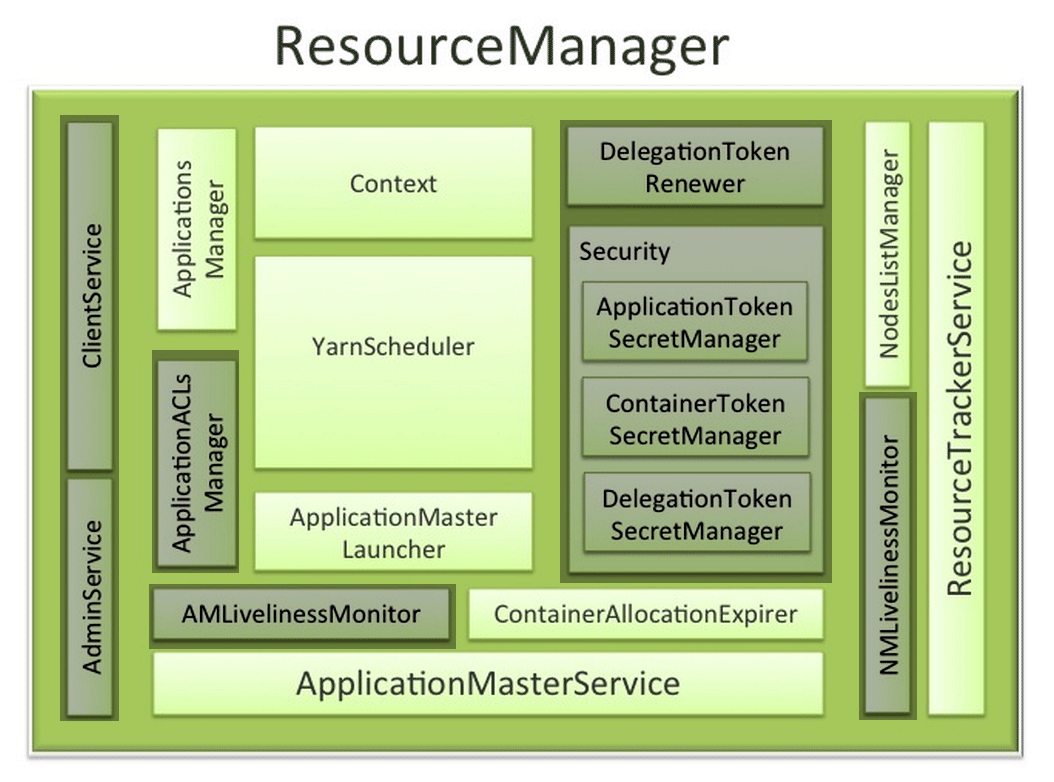
\includegraphics[width=15cm]{figuras/Figura14-RMHorton.png}
   \caption{ResourceManager Component Diagram \cite{HortonRM}}
   \label{fig:RMHorton}
\end{figure}

The ResourceManager is the master that arbitrates all the available cluster resources and thus helps manage the distributed applications running on the YARN system. It works together with the per-node NodeManagers (NMs) and the per-application ApplicationMasters (AMs) \cite{HortonRM}.

Except the scheduler itself, there are other components of fundamental importance to the scheduling process. Like the ApplicationsManager, which manages all the submitted applications. The ApplicationsManager component not only has a list of submitted applications, but also has information about all the completed applications and is able to provide this through either web UI or command line.

Another important component is the ApplicationMasterLauncher, that will be responsible to create the application specific ApplicationMaster, everytime an application is submitted. Another task left to the ApplicationMasterLauncher component is the deletion of ApplicationMaster when the application has finished, either normally of forcefully.

The ApplicationMaster itself is a concept that makes YARN completely different than the previous Hadoop versions. It is a key component on MapReduce tasks execution because it has one instance for every application being executed, making the ApplicationMaster the component responsible for the execution and monitoring of the containers and their resource consumption. Therefore, it has to communicate with the ResourceManager in order to ask and report the status and progress of its monitored containers.

It is through ApplicationMaster that YARN can achieve better scalability, since it takes some of the processing usually delegated to the Scheduler and ResourceManager components. One of the key tasks that was transferred to the ApplicationMaster is the fault tolerance. It is the ApplicationMaster that will decide when and/or if a speculative task is necessary and beneficial. Thanks to this shift in the responsibilities and the ApplicationMaster being a per-application manager, the cluster scaling potential is improved through the removal of a possible bottleneck. 

Another crucial component to the present work is the ResourceTrackerService, that is responsible for the communication with the NodeManagers. This is the component that answers to the RPC calls, whenever a node wants to register with the RM, send a heartbeat, or many other tasks, this is the component that will be used. The node capacity is also passed on the registration of a node with the RM, this process of registration will store the node's information in the NodesListManager. The second component is a collection of all the nodes, both the valid and the decomissioned ones.

Finally, the Scheduler follows the same pattern as regular scheduler, comparing requests, availabilities and then granting the resources based on some heuristic. However, most Hadoop schedulers use queues in order to help the task of managing the users and application submitted.

The other high level view that interests this work is the NodeManager. Just as the ResourceManager counterpart, even having some irrelevant modules presented in the figure \ref{fig:NMHorton}, it facilitates the understanding of the service in a high level. Having a high level understanding is necessary in order to understand how the two services will interact.

\begin{figure}[hbtn]
   \renewcommand{\figurename}{Figure}
   \centering
   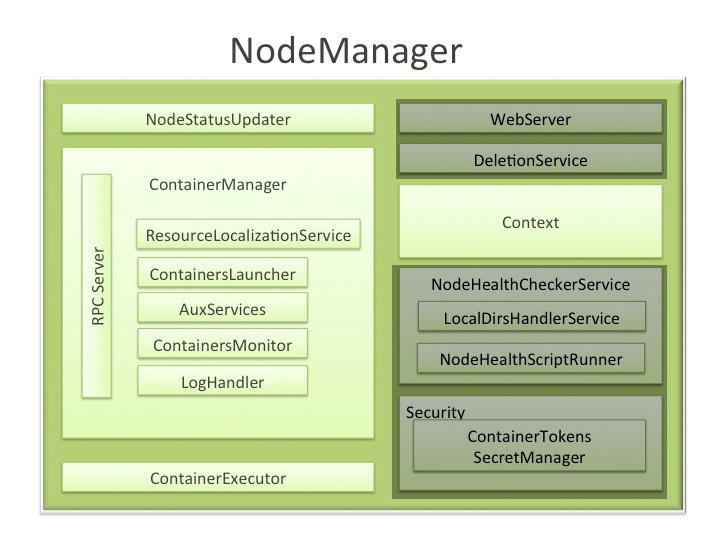
\includegraphics[width=15cm]{figuras/Figura15-NMHorton.png}
   \caption{NodeManager Component Diagram \cite{HortonNM}}
   \label{fig:NMHorton}
\end{figure}

Each slave will have a NodeManager instance running, which is the local manager. This service main responsibility is keeping his information updated on the ResourceManager, but it has other attributions like managing the containers, monitoring the resource usage, monitoring node health, among others.

One key component is the NodeStatusUpdater, which will be responsible for the registration with the ResourceManager, it is through registration that the ResourceManager will be informed about the resources of a given node, making this component vital for the success of the approach in this work. Also, after the initial registration this component is expected to maintain the communication with the ResourceManager in order to provide updates on containers launched, running or completed.

The largest component in the figure, the ContainerManager is as important as its size implies. With help from its sub-components, the ContainerManager has the hard but extremely necessary task of monitoring containers and informing whatever component needs this information. There are several ContainerManager sub-components, they are: RPC server, ResourceLocalizationService, ContainersLauncher, AuxServices, ContainersMonitor and LogHandler. Some like the ResourceLocalizationService is of vital importance to the MapReduce tasks, as it downloads the files that will be used on the tasks' execution, but won't interfere in this work's context.

The next diagram used to better understand the architecture was the scheduler components class diagram, which provided a helped to view classes related to the scheduling process. The Scheduler Components Class Diagram can be visualized in the figure \ref{fig:SchedCD}.

\begin{figure}[hbtn]
   \renewcommand{\figurename}{Figure}
   \centering
   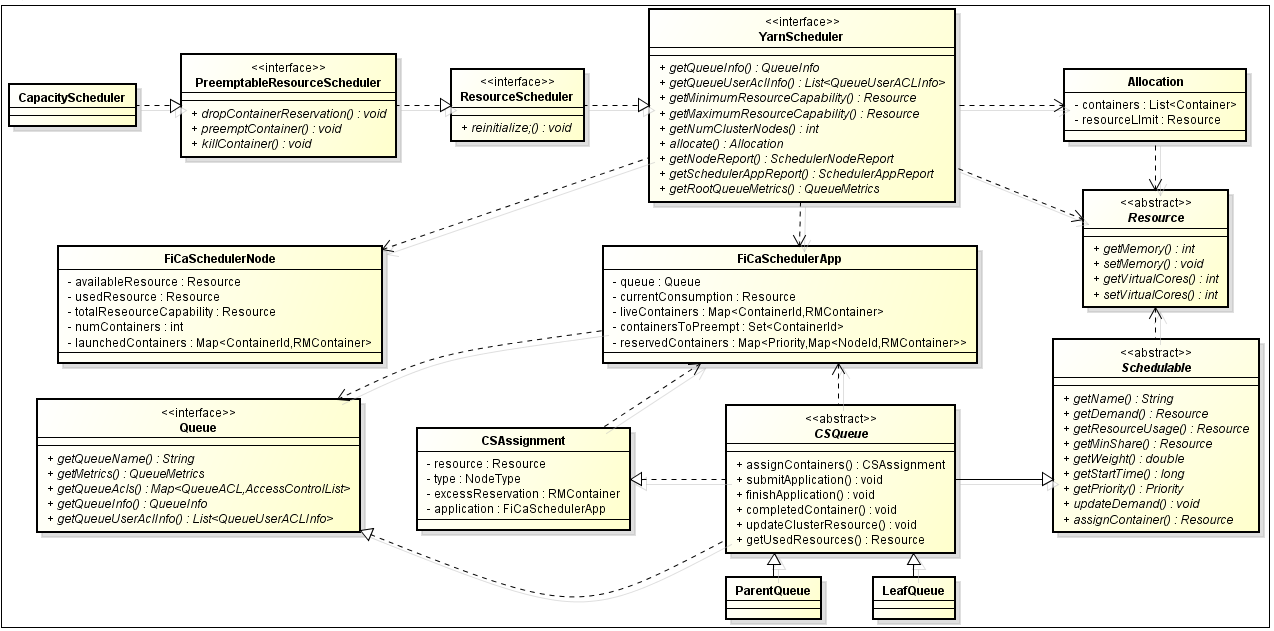
\includegraphics[width=15cm]{figuras/Figura01-ClassDiagram.png}
   \caption{Class Diagram with the main CapacityScheduler classes}
   \label{fig:SchedCD}
\end{figure}

Following is a description of the main components that compose the CapacityScheduler:
\begin{itemize}
	\item Schedulable: an abstract class that represents an entity capable of launching either a job or a queue, it offers a simple interface whereby the algorithms can be applied either inside a queue as well as several queues.
	\item Queue: an interface that enables the basic control of all the queues in the scheduler. Possessing methods to allow reading of the queue info, and also queue management.
	\item PreemtableResourceScheduler: another interface that allows the preemption of resources, through the scheduler.
	\item Resource: an abstract class responsible for modelling the resources capable of being use, which at this moment are only memory and core count.
	\item FiCaSchedulerNode and FiCaSchedulerApp: representations of the node and application, provides vital information about the structures. Uses a lot of the components present on the next Class Diagram.
\end{itemize}

Another key class diagram to the context of this work was the diagram that would represent three very important components, the RMContainer, RMNode and RMApp/RMAppAttempt. All of these components represents fundamental parts on understanding how this work has impacted the scheduling. RMContainer is the name given to the reservations of resources, making it also responsible for the task execution. RMNode is the representation of a whole NodeManager to the scheduler, and is through it that the scheduler will get access to the NodeManager real resource capacity. RMApp and RMAppAttempt represents the applications sent to the scheduler. This diagram is represented in the figure \ref{fig:RMComponents}.

\begin{figure}[hbtn]
   \renewcommand{\figurename}{Figure}
   \centering
   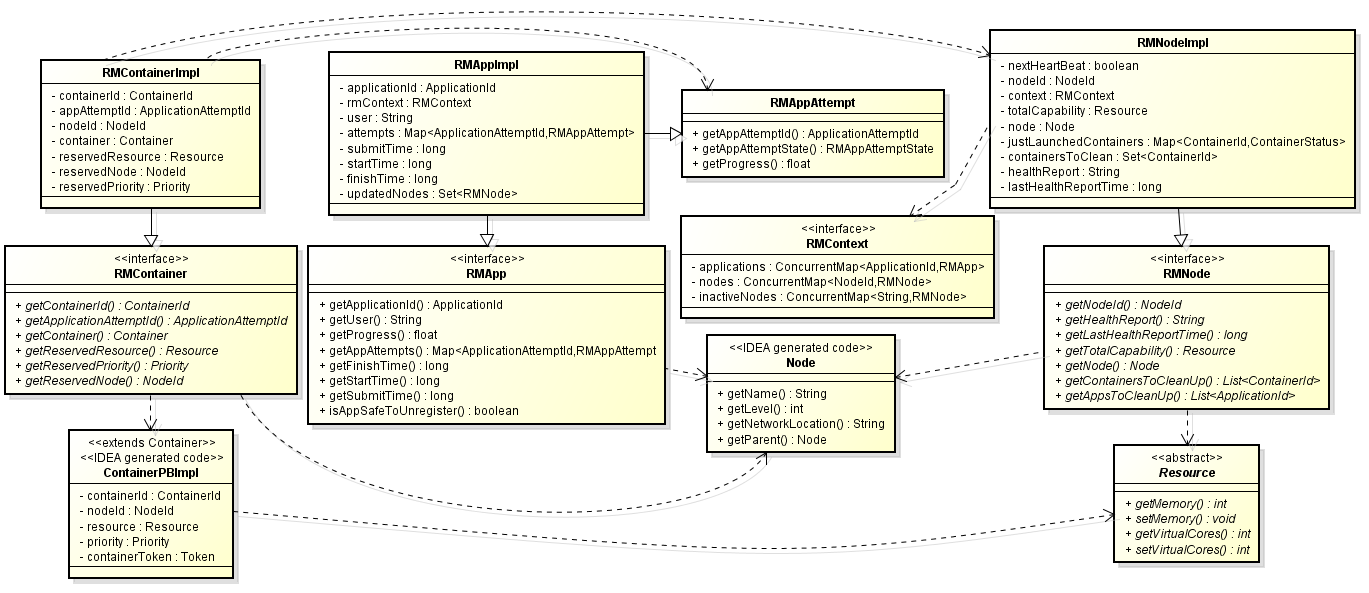
\includegraphics[width=15cm]{figuras/Figura13-RMComponents.png}
   \caption{Class Diagram with the main RM components}
   \label{fig:RMComponents}
\end{figure}

\subsection{State machines}

The second method was executed through an option offered by the Maven tool, in which it is possible to generate graphs that represents the Resource Manager and Node Manager state machines. Through analysis of the graphs it is possible to identify the life cycle of some key components, such as RMContainers, RMNodes and RMApplications. 

The importance of RMContainers, RMNodes and RMApplications may be overlooked until further analysis of source code and state machines at the same time. It is not a coincidence that all the components have a RM, referencing ResourceManager, in their names. In a brief explanation, RMNodes have all resource and other static information concerning a given NodeManager. RMContainers are the structures that represent the reservation of resources and also responsible for the processing. Finally, the RMApplication is the component that provides ResourceManager a way to access application status, reports and updates. All state machines and a more thorough explanation can be found on \autoref{chap:ApendA}.

%-------------------------------------------------------------------

\section{Understanding Hadoop allocation pattern}
\label{sec:alloc}
In order to improve Hadoop resource utilization and change the resource allocation behavior, it was necessary to understand how the allocation is made. That implies knowing and understanding the whole process of requisition and grant of resources, which is essentially the scheduling. After the experiments made with the objective of understanding this process, it was possible to identify which parameters influenced and how much impact would these parameters have once they were changed.

Once a quick research on official documentation and the parameters which can be set on XML files was made, it was found that there are five parameters that influence the allocation pattern for each resource. These parameters can be roughly divided into three classes: application request, cluster configuration towards containers and cluster configuration towards ApplicationMaster (AM). All of these parameters have default values in case the application did not set a request value or the cluster administrator did not set them properly on configuration files.

The application request parameters are set through the JobConf class when the user is coding his MapReduce job. If the parameters are not set at this time, the cluster will use the properties \textit{mapreduce.map.memory.mb} and \textit{mapreduce.reduce.memory.mb} either at the \textit{mapred-site.xml} or \textit{mapred-default.xml}, following default Hadoop behavior towards settings in the xml files. The default behavior is: if the properties are set in any \textit{*-site.xml} file that's the value they will assume, otherwise the values will be taken from \textit{*-default.xml} file.
The default value for properties \textit{mapreduce.map.memory.mb} and \textit{mapreduce.reduce.memory.mb} is 1024.

The cluster configuration towards containers is composed by four parameters, these parameters express the floor and ceiling of valid allocations. The floor limit parameters receive their values from the properties \textit{yarn.scheduler.minimum-allocation-mb} related to the memory and \textit{yarn.scheduler.minimum-allocation-vcores} related to the cores, while the ceiling limit parameters receive their values from properties \textit{yarn.scheduler.maximum-allocation-mb} and \textit{yarn.scheduler.maximum-allocation-vcores}. All properties will follow the default Hadoop behavior towards settings in XML files. These four parameters are related to two variables in the source code, which are named \textit{minimumAllocation} and \textit{maximumAllocation}, which represents the floor and ceiling limit respectively. 
The default value for \textit{yarn.scheduler.minimum-allocation-mb} is 1024 and the default value for  \textit{yarn.scheduler.minimum-allocation-vcores} is 1. The default values concerning the ceiling properties is 8192 for \textit{yarn.scheduler.maximum-allocation-mb} and 32 for \textit{yarn.scheduler.maximum-allocation-vcores}.

The only parameter left is the AM request, this request will be the same for every application submitted to the cluster and cannot be configured through JobConf. This parameter will receive it's value from properties \textit{yarn.app.mapreduce.am.resource.mb} related to the memory and \textit{yarn.app.mapreduce.am.resource.cpu-vcores} related to the cores, also following the default Hadoop behavior. The default value of the parameter \textit{yarn.app.mapreduce.am.resource.mb} is 1536, and, the default value of the parameter \textit{yarn.app.mapreduce.am.resource.cpu-vcores} is 1.

\subsection{Experiment}
In order to understand how the allocation process is made an experiment was performed. The experiment was made aiming to understand how the RM allocates memory for applications given requisition and minimum/maximum parameters changes. It consisted in altering some of the parameters and analysing the resultant behavior. As the AM request is the same across the cluster, it was excluded from the experiment. The reason being that different applications would have the same amount requested by the AM and it's behavior follows the same pattern as the other requests, which are easier to manipulate.

\subsubsection{Employed methods, procedures and scenarios}
The experiment was performed in a cluster deployed on Grid'5000 environment. The cluster had five nodes, one master and four slaves, each node having the following configuration: 2 CPUs AMD@1.7GHz, 12 cores/CPU and 47GB RAM. All nodes were running an Ubuntu-x64-1204 standard image, having Sun JDK 1.7 installed. The Hadoop distribution was the 2.2.0 YARN version.

The procedure chosen as data acquisition method was the Hadoop Log System. The reason for such a choice was that Hadoop Log System is, by default, enabled in the INFO level and using the INFO level would be possible to insert small entries and extract useful information in real time.

Following there is a brief description of the four scenarios used in the experiment:

\begin{itemize}
	\item \textbf{Default scenario}: no parameter was changed.
	\item \textbf{Requisition higher than maximum}: the application requested an amount of memory higher than the cluster maximum allocation parameter. The changed value was the maximum allocation memory. The minimum was also changed for consistency reasons.
	\item \textbf{Requisition smaller than minimum}: the application requested an amount of memory smaller than the cluster minimum allocation parameter. The changed value was the minimum allocation memory.
	\item \textbf{Requisition inside range}: the application requested an amount of memory inside the cluster valid range. The changed values were the minimum allocation memory and requisition from both map and reduce.
\end{itemize}

\subsubsection{Results and interpretation}

The results from the scenarios can be analysed on the table \ref{tab:memory allocation}.

\begin{table}
	\renewcommand{\figurename}{Table}
	\centering
	\begin{tabular}{|l|c|c|c|c|}
		\hline 
		Parameters & Default & Higher & Smaller & Inside\\ 
		\hline 
		Map Memory Requisition (MB) & 1024 & 1024 & 1024 & 3456\\ 
		\hline 
		Reduce Memory Requisition (MB) & 1024 & 1024 & 1024 & 3712\\ 
		\hline 
		Minimum Memory (MB) & 1024 & 512 & 2048 & 512\\ 
		\hline 
		Maximum Memory (MB) & 8192 & 768 & 8192 & 8192\\ 
		\hline 
		Map Memory Allocation (MB) & 1024 & ERROR & 2048 & 3584\\
		\hline
		Reduce Memory Allocation (MB) & 1024 & ERROR & 2048 & 4096\\ 
		\hline 		
	\end{tabular}
	\caption{RM memory allocation pattern experiment results}
	\label{tab:memory allocation}
\end{table}

%\begin{figure}[!hbtn]
%   \centering
%   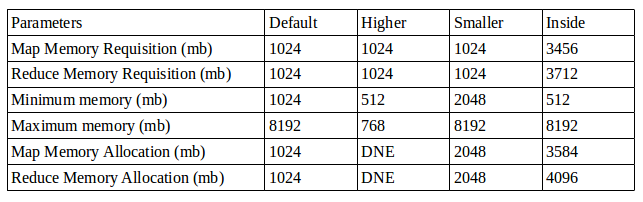
\includegraphics[width=15cm]{figuras/Figura09-allocation.png}
%
%\end{figure}

Because of the experiment, it was possible to detect that Hadoop allocation pattern differs a bit from usual. Unlike usual pattern in which if a request is inside the minimum and maximum range, the amount granted is equal to the request, the requests on Hadoop will pass through a small set of calculations in order to determine how much memory will be granted.

The figure \ref{fig:fluxoAllocation} portraits the  flow of operations executed by the Hadoop in order to determine the granted resources.

\begin{figure}[!hbtn]
   \renewcommand{\figurename}{Figure}
   \centering
   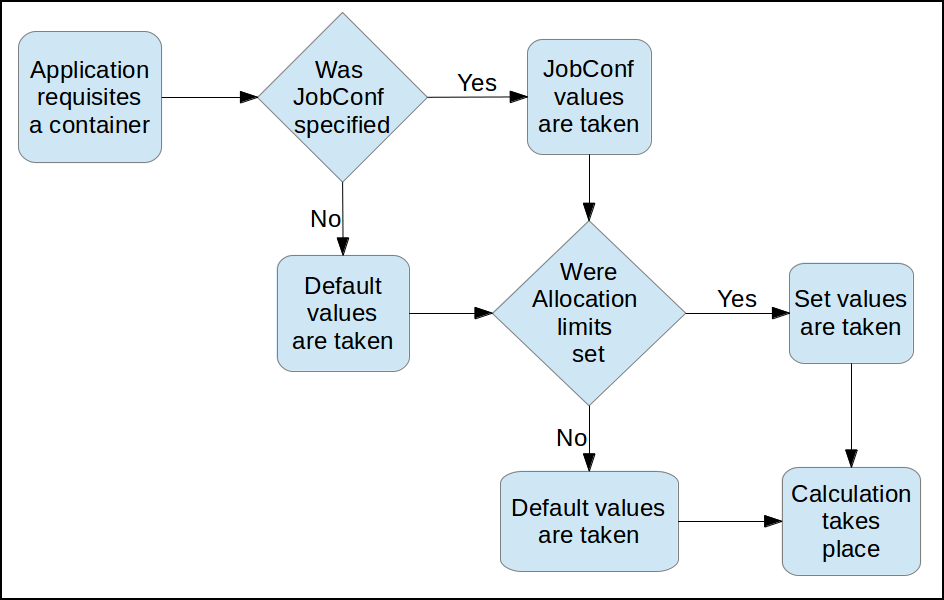
\includegraphics[width=15cm]{figuras/Figura18-allocflow.png}
   \caption{Flow of operations for resource granting}
   \label{fig:fluxoAllocation}
\end{figure}

The default scenario just demonstrates how Hadoop allocation will behave in case there are no interventions.

The second scenario shows what happens if the application requests a value higher than the maximum. The output is an error message and the job execution is aborted.

The third scenario shows what happens if the application requests a value smaller than the minimum. The cluster grants the minimum allowed.

The fourth scenario shows a case in which the requests are inside the valid range but although the requests were similar, the resources granted were different. This scenario is the one that makes it possible to fully comprehend the allocation process. Since the second and third scenarios provided evidence that a request can't be higher than the maximum and that at least the minimum allocation will be given, it is possible to infer that the allocation will always start with the minimum allocation value. In the case the minimum allocation is not enough to satisfy the request, the value which will be granted is always incremented by the minimum allocation until it matches one of the following cases: the value is equal to the request, the value is higher than the request and lower than the maximum allocation or the value exceeds maximum allocation. Concerning the scenario, it is the second case that occurs.

The figure \ref{fig:fluxoAllocation2} is provided along with extensive explanation to facilitate the understanding of the whole calculation process. 

\begin{figure}[!hbtn]
   \renewcommand{\figurename}{Figure}
   \centering
   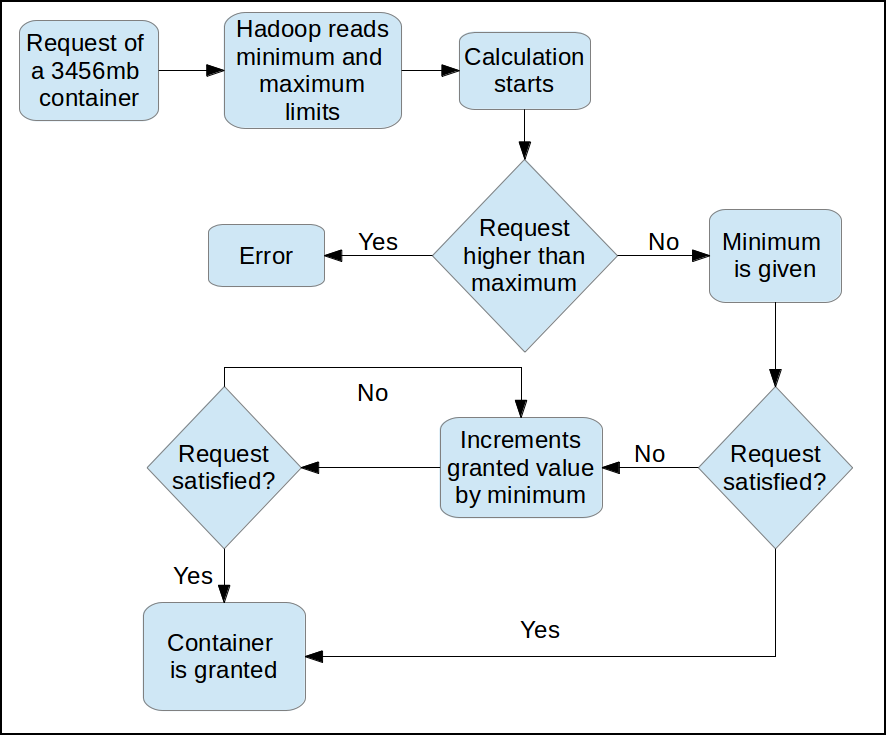
\includegraphics[width=15cm]{figuras/Figura19-allocflow2.png}
   \caption{Flow of operations for resource granting}
   \label{fig:fluxoAllocation2}
\end{figure}

The step by step calculation on scenario four will be demonstrated. Assuming M is the memory granted, or in the process of calculation, for the map request and R for the reduce. The calculation happens as follows:

Firstly the M and R are set to the minimum memory allocation property, which is 512. Since 512 does not satisfy any of the requests the M and R values are then incremented by the minimum memory allocation, assuming the value of 1024. As 1024 still smaller than both requisitions, they are again incremented by 512 and the process goes on as following:

M: 512, 1024, 1536, 2048, 2560, 3072, 3584.

R: 512, 1024, 1536, 2048, 2560, 3072, 3584, 4096.

Note that in both cases the value granted was the smallest multiple of minimum memory allocation (512) greater than or equal to the request (3456 and 3712).

%-------------------------------------------------------------------

\section{Context-aware scheduling}
Knowing that the scheduling task is closely related to the resources availability and, therefore, having a wrong information could ruin the performance of the algorithm, an opportunity for improvement was seen. After a quick study on the default schedulers, it was clear that CapacityScheduler already had the whole structure to support a better scheduling, as stated in the section \ref{sec:Hadoop Schedulers}. The flaw on CapacityScheduler wasn't really a scheduling flaw, but actually a wrong information received by the NodeManagers.

As stated numerous times in previous sections, Hadoop configuration is heavily dependent in XML files. While providing an easy way to configure a real cluster, sometimes it acts more as an obstacle than as a facilitator, the reason being that if one wants to change a parameter the whole service will have to be restarted. One huge restriction implied by XML files, is regarding the nodes capacity. In case one doesn't want to use Hadoop default configurations for node capacity, every node will have to have it's XML files edited. In a large heterogeneous cluster, modifying one file in each node will certainly be time consuming since each node will have a different configuration. 

One possible solution to this case, is to overwrite the value gotten from XML file on the code. At first glance this brings in more problems than solutions, because the administrator would have to chose a certain hard coded value that would fit best as an average among all nodes. However, as one looks closer into the proposal, there is an option that, although involving more coding, would solve this problem. 

It is clear that this solution requires the application to detect some context of the environment. The context, in this case, being the real information about node capacity. With this context at hands, it is a reasonable choice to make the scheduler context-aware. Therefore, improving the scheduling performance. As the section \ref{sec:ctx} implies, being context-aware requires the application to detect and adapt to changes in environment.

Regarding the detection of the node capacity, the chosen option was to integrate a collector into Hadoop, meaning that every node would be able to access it's true capacity. Thus, preventing the hard coding that was suggested.

Regarding the changes made once the context information was detected, the approach adopted was to scale the allocation limits together with the total cluster resource availability. This scaling meant that the containers would have more memory and cores at their disposal and, therefore, speculative task would hardly have to be launched. Also, by adapting to the cluster real resource, no resource would be wasted or left inactive while the scheduler is making tasks wait due to wrong information being received. Thus improving the cluster utilization.

\subsection{Collector description}
The collector of choice was PER-MARE's collector \cite{Collector}. This collector uses a standard java package in order to access the real node capacity, therefore, no additional libraries would be necessary.
 
Only four files were necessary, an interface, an abstract class and two classes. Due to it's design, it would be easy to integrate new collectors and improve the resources available for the scheduling process, providing data about the CPU load or disk usage for example.

The base of the collector is the interface Collector, which has two access methods and the collect method. 

The abstract class, called AbstractOSCollector, implements the interface and has some access methods of its own. The great usability comes from the usage of OperatingSystemMXBean, a public java interface that is used to access the operating system informations on which the Java virtual machine is running \cite{MXBean}.

The collector classes, called PhysicalMemoryColletor and TotalProcessorsCollector extends the AbstractOSCollector and have only constructor and collector method implemented.
%TODO trechos de c´odigo no appendix?

\subsection{Collector integration with Hadoop}
The collector would have to be placed on NodeManager (NM), since this is the service responsible for processing tasks. The collected capacity is then sent to the ResourceManager (RM) in the moment that each NM is registering with the RM. It is possible to view the whole process of data acquisition until CapacityScheduler add the node in the figure \ref{fig:collectorflow}.

\begin{figure}[!hbtn]
   \renewcommand{\figurename}{Figure}
   \centering
   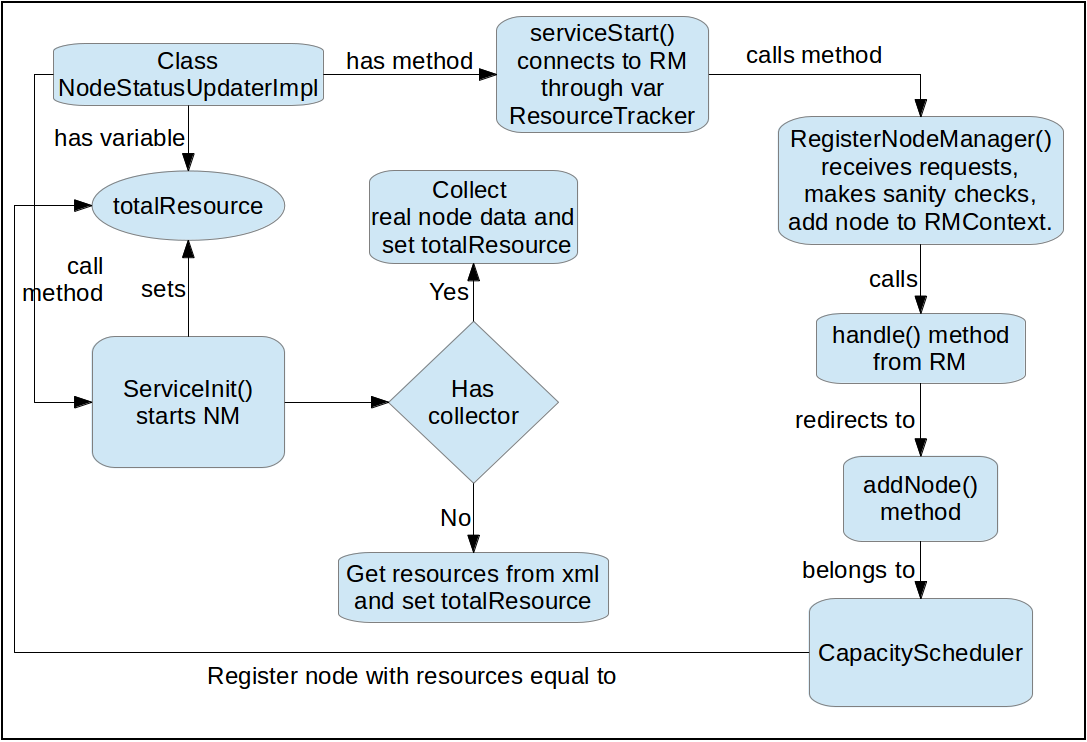
\includegraphics[width=15cm]{figuras/Figura20-collectorfig.png}
   \caption{Flow of operations for resource granting}
   \label{fig:collectorflow}
\end{figure}

After the collector integration, changing the scheduling behavior was possible due to the now available information about the real resources of a given node. Further information about the results gotten from the collector integration and modified scheduling can be found at the chapter \ref{chap:Experiments and Results}.
\chapter{Próximas Etapas}
%-------------------------------------------------------------------
As próximas etapas deste projeto são as seguintes:
\begin{enumerate}
   \item Decisão das métricas do algoritmo de escalonamento com base nos recursos identificados e suportados pelo \emph{Hadoop}
   \item Implementação do escalonador
   \item Testes e avaliação
   \item Ajustes e novos testes se necessário
\end{enumerate}


\setlength{\baselineskip}{\baselineskip}

%%=============================================================================
%% Referências
%%=============================================================================
\bibliographystyle{abnt}
\bibliography{referencias/referencias}



%IMPORTANTE: Se precisar usar alguma seção ou subseção dentro dos apêndices ou
%anexos, utilizar o comando \tocless para não adicionar no Sumário
%Exemplos: 
% \tocless\section{Histórico}
%%=============================================================================
%% Apêndices
%%=============================================================================
\appendix

\chapter{Grafos gerados referentes ao \emph{ResourceManager}}
\label{chap:ApendA}

A seguir encontram-se uma breve explicação e as figuras geradas pelo segundo método empregado na etapa de estudo da arquitetura do \emph{framework}.

A pertinência das figuras é validada por elas descreverem todos os caminhos possíveis que dada interface pode tomar. O fluxo do caso perfeito seria iniciado com o recebimento de um novo \emph{job} pelo \emph{ResourceManager}. Para que o \emph{job} possa ser iniciado alguns pré-requisitos devem ser satisfeitos. É a partir desse ponto que as figuras entram em cena.

Para que uma aplicação seja iniciada, primeiramente é criado um \emph{AppAttempt}. O \emph{AppAttempt} é literalmente uma tentativa de aplicação, pela qual o \emph{ResourceManager} tentará alocar os recursos necessários (\emph{Node e Container}) para que essa aplicação seja realmente criada e submetida ao cluster. Durante o processo do \emph{RMAppAttempt} o \emph{ResourceManager} irá tentar alocar um ou mais \emph{RMContainers} bem como \emph{RMNodes} para que a aplicação tenha recursos suficientes para sua execução. Após os recursos necessários terem sido alocados com sucesso, a aplicação passa para o status de \emph{RMApp} e é submetida ao cluster.

%IMPORTANTE: Se precisar usar alguma seção ou subseção dentro dos apêndices ou
%anexos, utilizar o comando \tocless para não adicionar no Sumário
%Exemplos: 
% \tocless\section{Histórico}
% \tocless\subsection{Detalhes}
%\tocless\section{teste}
%Este é um teste de seção dentro do apêndice

\begin{figure}[hbtn]
   \centering
   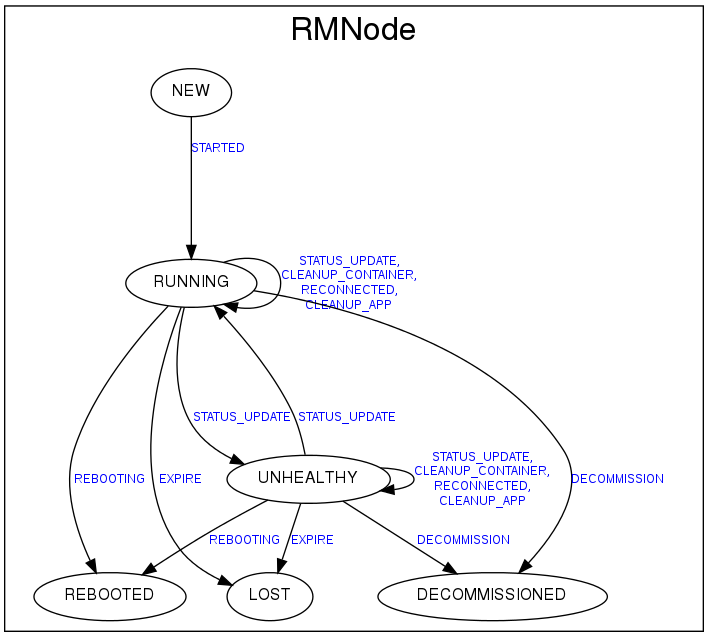
\includegraphics[width=12cm]{figuras/Figura05-RMNode.png}
   \caption{Máquina de estados do RMNode}
   \label{fig:RMNode}
\end{figure}

\begin{figure}[hbtn]
   \centering
   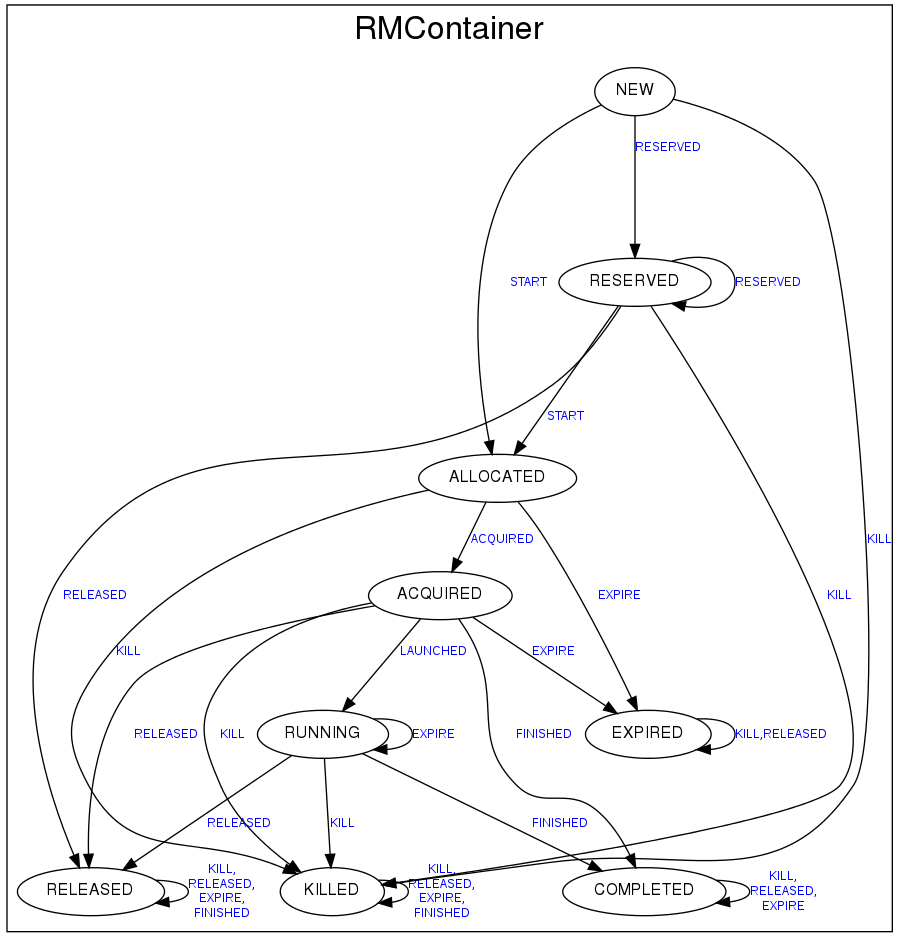
\includegraphics[width=15cm]{figuras/Figura03-RMContainer.png}
   \caption{Máquina de estados do RMContainer}
   \label{fig:RMContainer}
\end{figure}

\begin{figure}[hbtn]
   \centering
   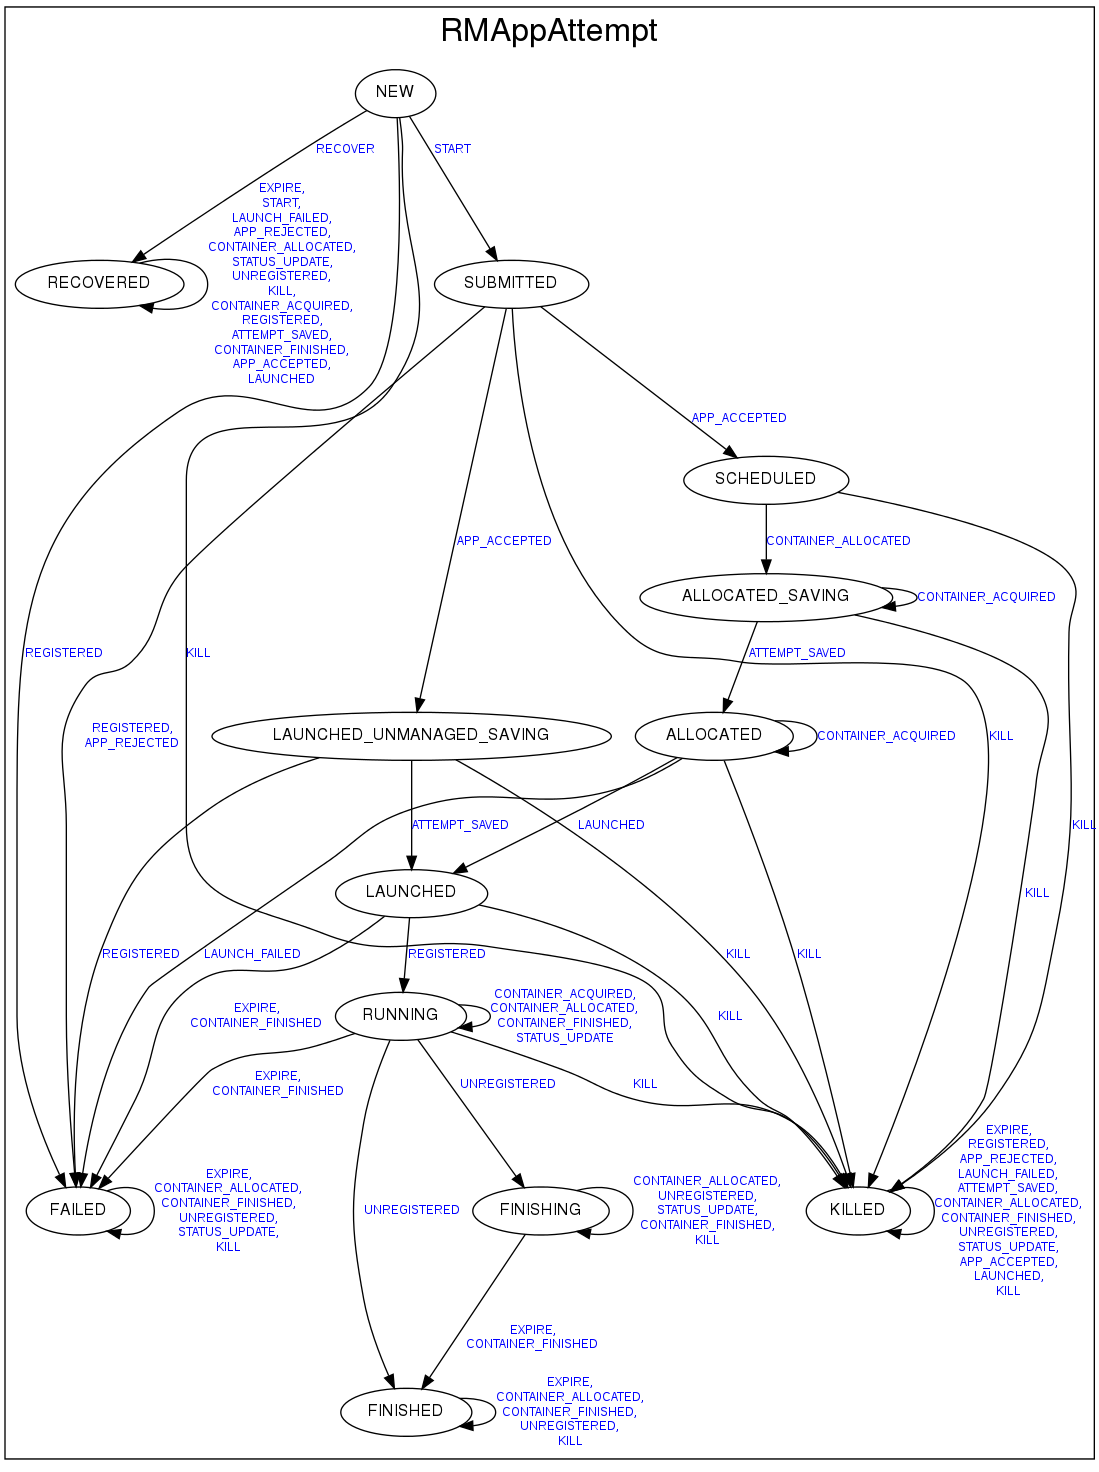
\includegraphics[width=15cm]{figuras/Figura02-RMAppAttempt.png}
   \caption{Máquina de estados do RMAppAttempt}
   \label{fig:RMAppAttempt}
\end{figure}

\begin{figure}[hbtn]
   \centering
   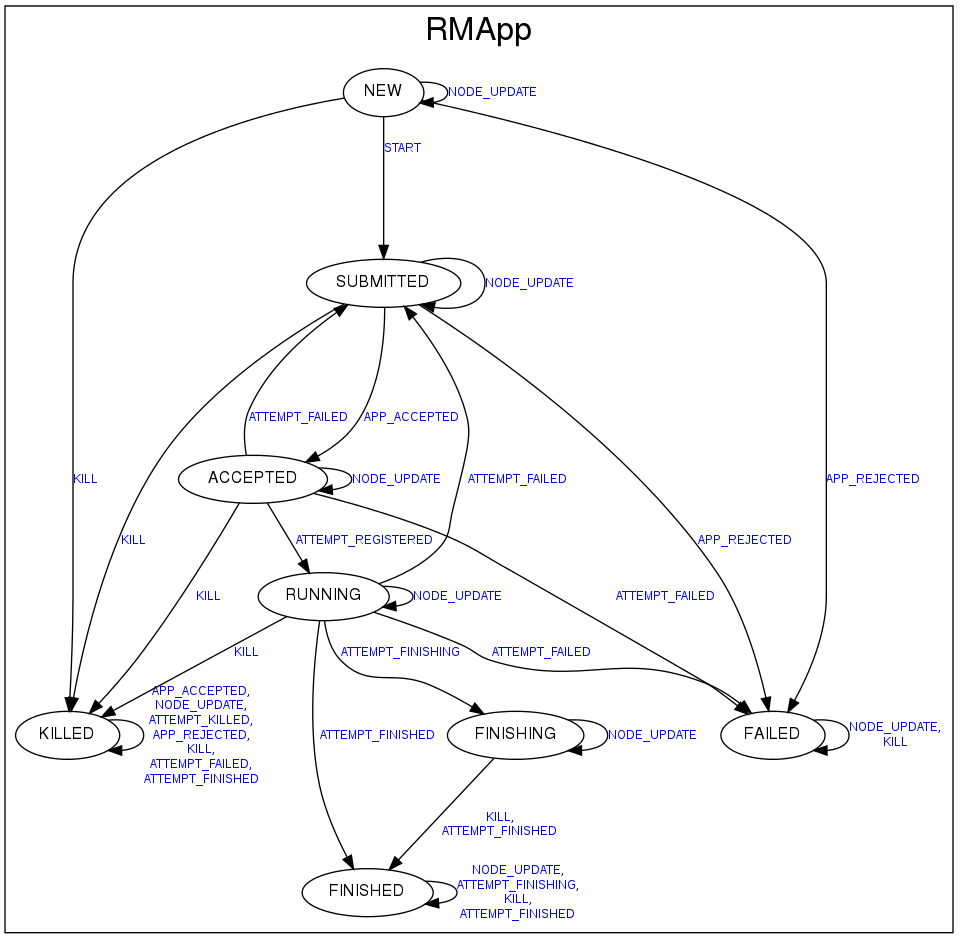
\includegraphics[width=15cm]{figuras/Figura04-RMApp.png}
   \caption{Máquina de estados do RMApp}
   \label{fig:RMApp}
\end{figure}
%
\chapter{Título do apêndice Ex}
Esta é o apêndice B



%%=============================================================================
%% Anexos
%%=============================================================================
%\annex
%
\chapter{Questionários aplicados para a Análise de Tarefas}



%
\chapter{Resultados da Análise de Casos de Uso}
\begin{figure}[hbtn]
   \centering
   \includegraphics[width=6.5cm]{figuras/figura09-anexob.eps}
   \caption{Análise dos pincipais Portais da área de Informática de instituições federias}
   \label{fig:CASOSDEUSO}
\end{figure}

\end{document}
